Программный модуль media scanner осуществляет нахождение медиа-файлов (аудио, видео, изображение) и извлечение мета-данных с записью их в XML-формат. Данный программный модуль не соответствовал следующим условиям, при которых система распознает его как плагин:
\begin{itemize}
  \item директория для временных файлов /tmp;
  \item исходный код должен находится в папке /src;
  \item *.pro файл должен именоваться Task*.pro;
  \item файлы *.cpp и *.h должны соответствовать шаблону TaskExample.
\end{itemize}

После выполения данных условий система <<COEX>> успешно распознает, собирает (рис.~\ref{ship_6:ship_6}) и выполняет данный плагин (рис.~\ref{ship_7:ship_7}). Результат выполнения программного модуля представлен на рисунке~\ref{ship_8:ship_8}.

\begin{figure}[h!]
\center{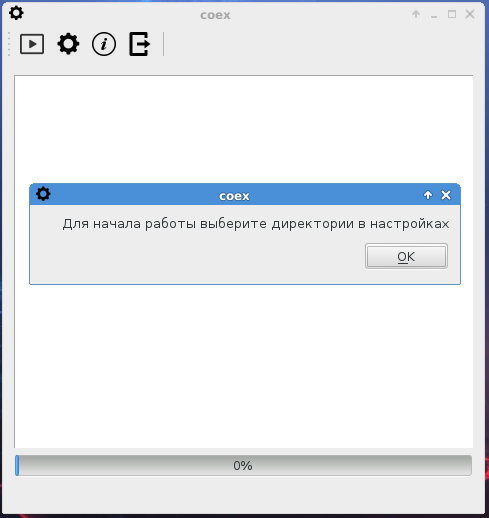
\includegraphics[width=0.5\linewidth]{ship_6}}
\caption{ Успешная сборка плагина }
\label{ship_6:ship_6}
\end{figure}

\begin{figure}[h!]
\center{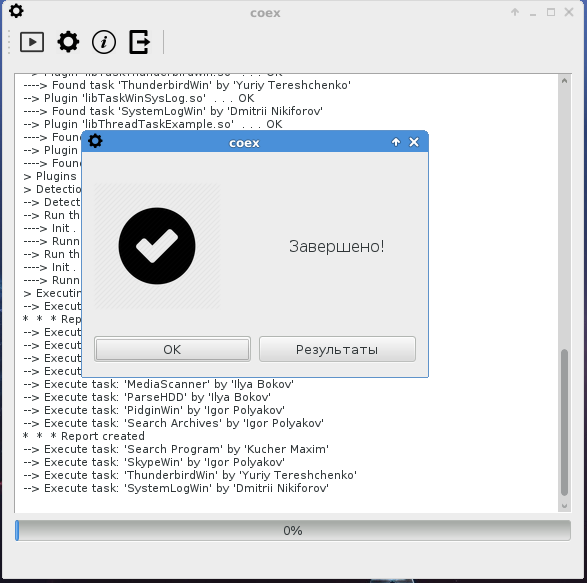
\includegraphics[width=0.7\linewidth]{ship_7}}
\caption{ Выполнение плагина }
\label{ship_7:ship_7}
\end{figure}

\begin{figure}[h!]
\center{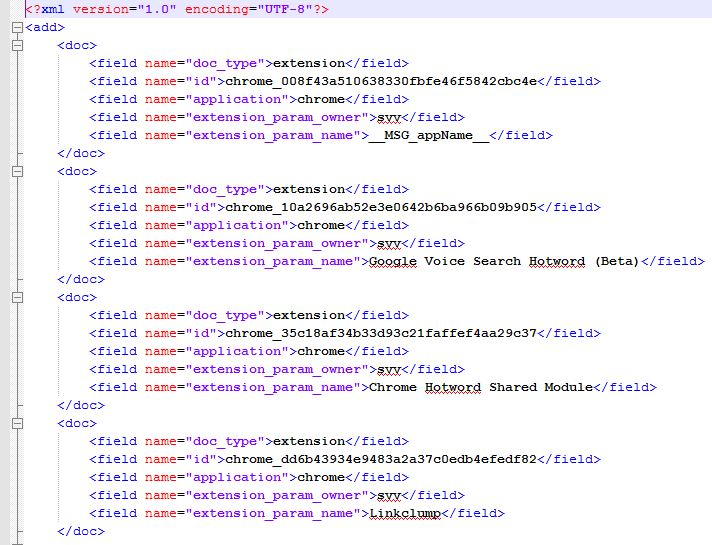
\includegraphics[width=0.9\linewidth]{ship_8}}
\caption{ Результат выполнения плагина }
\label{ship_8:ship_8}
\end{figure}

\clearpage
